\documentclass[%
 aip,
% jmp,
% bmf,
% sd,
% rsi,
cp,  % Conference Proceedings
 amsmath,amssymb,%nobibnotes,
% preprint,%
 reprint,%
%author-year,%
%author-numerical,%
]{revtex4-2}

\usepackage{graphicx}% Include figure files
\usepackage{dcolumn}% Align table columns on decimal point
\usepackage{bm}% bold math
%\usepackage[mathlines]{lineno}% Enable numbering of text and display math
%\linenumbers\relax % Commence numbering lines

\usepackage[utf8]{inputenc}
\usepackage[T1]{fontenc}
%% Loads a Times-like font. You can also load
%% {newtxtext,newtxtmath}, but not {times}, 
%% {txfonts} nor {mathtpm} as these packages
%% are obsolete and have been known to cause problems.
\usepackage{mathptmx} 
\usepackage{multirow}

\newcommand{\be}{\begin{equation}}
\newcommand{\ee}{\end{equation}}
\newcommand{\rf}[1]{(\ref{#1})}
\newcommand{\RR}{\mathbb{R}}
\newtheorem{thm}{Theorem}
\newtheorem{lm}{Lemma}

\begin{document}

\title{Comparison Between Two Numerical Methods for Solution of 2D Boussinesq Paradigm Equation}% Force line breaks with \\

\author{Angelow} % Write as First name Surname
 \email[Corresponding author: ]{angelow@math.bas.bg}
\affiliation{
Institute of Mathematics and Informatics\\
Bulgarian Academy of Sciences, Acad.\\
G.~Bonchev Bl.8, 1113, Sofia,
Bulgaria
}

\date{\today} % It is always \today, today, but any date may be explicitly specified
              % Not printed for conference proceedings

\begin{abstract}
In this paper we evaluate propagating wave solutions to the two dimensional Boussinesq Paradigm Equation (BPE).
Two numerical methods are used to obtain solution for the equation. The first is a Conservative Finite Difference Scheme (FDS), and the second exploits Taylor Series (TS) expansions around the time variable $t$. Furthermore, for each method the energy and the mass of the solution are calculated. The results, i.e. the solution, energy and mass, from the two methods are compared.
The solution is computed over three nested meshes to examine the convergence of both approaches. The energy and mass are found for each iteration step. In the case of the Conservative FSD the energy is computed using trapezoidal rule. In the case of TS the energy is calculated using trapezoidal, Simpson's and Boole's rules with $O(h^{2} + \tau^2 )$, $O(h^{4} + \tau^4 )$ and $O(h^{6} + \tau^6 )$ approximation errors, respectively. The main tool for testing the convergence rate $\xi$ of all examined finite difference schemes and TS expansions is the Runge's Method.
The goal is to justify the TS approach by showing that both methods produce similar results in case of $O(h^{2} + \tau^2 )$ approximation order. Furthermore, the TS method could be used with higher approximation order to produce finer results. The outcome of the comparison is very good. The maximum difference between the two approaches (among calculated solutions using different parameter sets) in $L_2$ and infinity norms is $0.009981$ and $0.004560$ respectively.
%here99 use percentage notation

\end{abstract}

\maketitle

\section{\label{sec:level1}Introduction}

The standard two dimensional BPE formulation was first derived in \cite{ref1}

\begin{align}\label{problemCh}
 \frac{\partial^2 u}{\partial t^2}= \Delta u + \beta_1 \Delta \frac{\partial^2}{\partial t^2} u -  \beta_2 \Delta^2 u +  \alpha \Delta (u^2)
\\
u(x,y,0) = u_0(x,y), \quad \frac{\partial u}{\partial t}(x,y,0)=u_1(x,y), \nonumber
\\
u(x,y,t) \rightarrow 0, \quad \Delta u(x,y, t) \rightarrow 0 \quad \text{for} \quad \sqrt{x^2+y^2} \rightarrow \infty \nonumber
\end{align}
where $\alpha>0$ is amplitude, $\beta_1>0$, $\beta_2>0$  are dispersion parameters, and $\Delta$ is the Laplace operator. The domain of the unknown function $u$ is defined by:
\be
 u:\Omega \times [0, T] \rightarrow R
\ee
where $\Omega \equiv \RR^2$ and $T>0$. For the numerical interaction of 2D Boussinesq traveling waves (TW) one needs the shape of a stationary wave in order to build the Initial Condition (IC) $u_0$, $u_1$. The stationary two dimensional wave, travelling in $y$ direction, with velocity $c$ is defined by
\be\label{ellipticSubst}
	U(x, y-ct) = u(x,y,t).
\ee
Without loss of generality the direction of motion is chosen along the positive $y$ axis. With a suitable variable change the direction could be rotated by an arbitrary angle in the 2D plane. If the substitution \rf{ellipticSubst} is applied in \rf{problemCh} then an eliptic partial differential equation is obtained. The last has been evaluated in many articles some of which are \cite{ref13}, \cite{ref14}, \cite{ref15} and \cite{ref16}. The first two \cite{ref13}, \cite{ref14} apply Galerkin method with an orthonormal function basis in $L^2(-\infty, \infty)$. The Perturbation Solution \cite{ref15} in 2D derives the "best fit" formula which is a series solution around small parameter - the wave speed $c$. Here one makes use of an exact formula which approximates the solution. The last article \cite{ref16} reflects the work that is done here. The TS approach with Method of Lines (or simply Taylor method) uses high order FDS along the spatial domain. In order to satisfy this requirement an IC with high order FDS is built in \cite{ref16}.

The 2D hyperbolic equation \rf{problemCh} is solved numerically in \cite{ref20}, \cite{ref21}, \cite{ref22} and \cite{ref23}. The most important observation is that all those papers (and many others) apply the "best fit" formula from \cite{ref15} with small wave speeds $c \approx 0.3$ to construct the IC and report that the wave either blows up or disperses in the form of ring wave expanding to infinity after some time period. Nevertheless, there are still no tests in the literature for solving \rf{problemCh} with IC for higher wave speeds $c^2 \approx min\{1, \frac{\beta_2}{\beta_1} \}$ and no tests with IC different from the perturbation solutions found in \cite{ref15}.

The goal of this work is to first, investigate high order accurate solutions to the BPE with new type of IC obtained in \cite{ref16} where the approximation order of the IC corresponds to the Taylor method applied here. Second, evaluate numerically the Mass, Energy, shape and maximum of the resulting waves for velocities, which are close to the maximum $c \approx c_{max}$, $c < c_{max}$ where $c_{max} = min\{1, \sqrt{ \frac{\beta_2}{\beta_1} } \}$. Third, show that the enumerated properties of the solution remain constant for some fixed time interval. Two numerical methods are applied to the BPE \rf{problemCh}, namely, a Conservative Finite Difference Scheme (FDS) and Taylor Series (TS) approach with Method of lines. There already exist results obtained by the Conservative FDS \cite{ref20}. The last is used as a referent mechanism. The Taylor method, on the other hand, is a novel approach when applied to the BPE. Results from both techniques are compared. The convergence speed is also investigated with respect to the type of approximation and solution style.

\section{Conservation of the Energy}

For convenience, the following variable change 
\begin{align}
x = \sqrt{\beta_1} \bar{x}, \quad y = \sqrt{\beta_1} \bar{y}, \quad t = \sqrt{\beta_1} \bar{t} \nonumber
\end{align}
is applied which transforms the main equation \rf{problemCh} into
\be\label{problemVC}
\beta(I-\Delta) \frac{\partial^2 u}{\partial t^2}= \beta \Delta u -\Delta^2 u -\alpha \beta \Delta (u^2)
\ee
where $\beta = \beta_1/\beta_2$. Define the operator $A$ as $Av=-\Delta_h v=-v_{\bar{x}x} - v_{\bar{y}y}$ and consider the FDS
\be\label{FDS1}
\beta (E+A)v_{\bar{t}t}^k +\beta Av^k+A^2 v^k -\alpha \beta A\left(\frac{(v^{k+1})^3-(v^{k-1})^3}{3(v^{k+1}-v^{k-1})} \right)=0
\ee
Multiply \rf{FDS1} by $A^{-1}$ and get 
\be\label{FDS2}
\beta (E+A^{-1})v_{\bar{t}t}^k +\beta v^k+A v^k -\alpha \beta \frac{(v^{k+1})^3-(v^{k-1})^3}{3(v^{k+1}-v^{k-1})} =0
\ee
Substitute $v^{k}=0.5(v^{k+1}+v^{k-1})-\frac{\tau^2}{2}v_{\bar{t}t}^k$ into \rf{FDS2}
and obtain
\begin{align*}
&\left( \beta (E+A^{-1})- \frac{\tau^2}{2}(\beta E+A ) \right)v_{\bar{t}t}^k  + \frac{1}{2} (\beta E +A )(v^{k+1}+v^{k-1}) \\
&~~~~~-\alpha \beta \frac{(v^{k+1})^3-(v^{k-1})^3}{3(v^{k+1}-v^{k-1})} =0
\end{align*}
Multiply the previous equation by $(v^{k+1}-v^{k-1})=\tau (v_{\bar{t}}^k + v_{t}^k)$ and sum over the spatial mesh points.
Reorganize the expressions to get the following formula 
\be \label{num_en}
E_h(v^k) =E_h(v^{k-1}),
\ee
where
\begin{align*}
E_h(v^k)=\left( \left( \beta (E+A^{-1})- \frac{\tau^2}{4}(\beta E+A ) \right)v_{t}^k ,v_{t}^k \right)+\frac{1}{4} \beta \left(  v^{k+1}+v^{k}, v^{k+1}+v^{k} \right) \\
+\frac{1}{4}  \left(  A(v^{k+1}+v^{k}), v^{k+1}+v^{k} \right)
-\alpha \beta \frac{((v^{k+1})^3,1)+((v^{k})^3,1)}{3}.
\end{align*}
In this way the following theorem is proved
\begin{thm}
The solution to the FDS \rf{FDS1} conserves the discrete energy
 $E_h(v^0)$, i.e.  $E_h(v^k) =E_h(v^{0})$ for each $k=1,2,...K$.
\end{thm}

\begin{thm}
The linear FDS corresponding to \rf{FDS1} is conditionally stable if
the following restriction is satisfied
$\tau^2 < \frac{\beta}{2}(1-\frac{\tau^2}{4}) h^2$.

\end{thm}
The proof is a consequence of the stability results from the book of
 Samarskii,  The theory of difference schemes, Marcel Dekker Inc., New York, 2001.

\section{Quadrature Formulas for the Mass and Energy}

The Mass of the continuous problem \rf{problemVC} is defined by
\begin{equation}\label{int}
D(u(t))=D(u(0))=\int_{\RR^2} u(x,y)dx dy
\end{equation}
and the Energy
\begin{align}\label{ex-en}
E(u):=&\int_{\RR^2} u_t \left((A^{-1}+E)u_t\right) dxdy+
\beta \int_{\RR^2} u^2 dxdy \nonumber\\
+& \int_{\RR^2}u \left(A u\right) dxdy
-\frac{2 \alpha \beta}{3} \int_{\RR^2} u^3 dxdy =const
\end{align}
where $Au=-\Delta u$. Here $E(u)$ is the exact energy of problem \rf{problemVC}.

At first, the unbounded domain is replaced by a sufficiently large computational domain $\Omega$. Then a uniform mesh $\Omega_h$ is defined in the following way
$$
\Omega_h = \{(x_i,y_j): x_i = ih, y_j = jh, i = 0,\cdots ,N_x, j = 0,\cdots , N_y \},
$$
where the discretization step $h$ satisfies $h = L_x/N_x = L_y/N_y$. The half size of $\Omega_h$ along $x$, $y$ directions is denoted with $L_x$, $L_y$. The time step is denoted with $\tau$. The value of the unknown function $u$ at mesh point $(x_i,y_j,t_k)$ is denoted with $u_{i,j}^k$, i.e. subscript is used for spatial discretization and superscript for time discretization.
Let us replace the operator $Au=-
\Delta u$ with discrete operators $-\Delta_h u$ with different approximation errors - $O(h^2)$, $O(h^4)$, $O(h^6)$. Suppose that the discrete approximation of the derivative $u_t$ is evaluated with approximation errors $O(\tau^2)$, $O(\tau^4)$, $O(\tau^6)$. Then one can apply quadrature formulas to evaluate numerically the energy \rf{ex-en}!

%When the numerical solution is found with $O(h^2+\tau^2)$ error, we apply \rf{quadr2} with $O(h^2)$ error;

%When the numerical solution is found with $O(h^4+\tau^4)$ error, we apply 2D Simpson's rule \rf{quadr4} with $O(h^4)$ error;

%When the numerical solution is found with $O(h^6+\tau^6)$ error, we apply 2D Boole's rule \rf{quadr6-2D} with $O(h^6)$ error;

Quadrature formulas in 2D case for evaluation of 

\begin{equation}\label{int}
D(u)=\int_{a_1}^{b_1} \int_{a_2}^{b_2} u(x,y)dx dy
\end{equation}

$x_i, ~i=0,1,...,N_x$; $x_0=a_1,~x_{N_x}=b_1$, $h_1=(b_1-a_1)/N_x$


$y_j, ~j=0,1,...,N_y$; $y_0=a_2,~y_{N_y}=b_2$,  $h_2=(b_2-a_2)/N_y$

\subsection{ 2D trapezoidal formula with global $O(h_1^2+h_2^2)$ error }

Let us assign the $X$ and $Y$ dimensions of the computational domain with $N_x$ and $N_y$. Then the approximation of the integral \eqref{int} 
with global $O(h_1^2+h_2^2)$ error is

\begin{align}\label{quadr2}
D_h(u_{i,j}) =& \sum_{i=1}^{N_x-1} \sum_{j=1}^{N_y-1} h_1 h_2 u_{i,j}
+\frac{h_1}{2}\sum_{i=0} \sum_{j=1}^{N_y-1} h_2 u_{i,j}
+\frac{h_1}{2}\sum_{i=N_x} \sum_{j=1}^{N_y-1} h_2 u_{i,j} \nonumber\\
+&\frac{h_2}{2}\sum_{j=0} \sum_{i=1}^{N_x-1} h_1 u_{i,j}
+\frac{h_2}{2}\sum_{j=N_y} \sum_{i=1}^{N_x-1} h_1 u_{i,j}
\nonumber\\
+&\frac{1}{4}h_1 h_2 \left(u_{0,0}+u_{N_x,0}+u_{N_x,N_y}+u_{0,N_y}
\right)
\end{align}

\subsection{ 2D Simpson's rule with global $O(h_1^4+h_2^4)$ error}

Here it is assumed that $N_x=2k$, $N_y=2 l$. For every $m=0,1,2,\cdots N_y$ it is computed that 
$$D_m= \frac{h_1 }{3} 
\left\{ u_{0,m}+u_{N_x,m}+ 4 \sum_{i=1}^{\frac{N_x}{2}}   u_{2i-1,m}
 +2 \sum_{i=1}^{\frac{N_x}{2}-1} u_{2i,m} \right\}.$$


Then 

\begin{equation}\label{quadr4}
D_h(u)=\frac{h_2 }{3} 
\left\{ D_{0}+D_{N_y}+ 4 \sum_{j=1}^{\frac{N_y}{2}}   D_{2j-1}
 +2 \sum_{j=1}^{{\frac{N_y}{2}}-1} D_{2j} \right\}
\end{equation}
is the approximation of the integral \eqref{int} with global $O(h_1^4+h_2^4)$ error


\subsection{ 2D Boole's rule with global $O(h_1^6+h_2^6)$ error }
Here it is assumed that $N_x=4k$, $N_y=4 l$. For every $m=0,1,2,\cdots N_y$ it is computed that

\begin{align*}
D_m =& \frac{2h_1}{45} 
\left\{
7u_{0,m}+7u_{N_x,m}+32 \sum_{i=1}^{\frac{N_x}{2}}u_{2i-1,m}
+12\sum_{i=1}^{\frac{N_x}{4}}u_{4i-2,m}
+14 \sum_{i=1}^{\frac{N_x}{4}-1}u_{4i,m}
\right\}.
\end{align*}


Then \eqref{quadr6-2D} is the approximation to the integral \eqref{int} with global $O(h_1^6+h_2^6)$ error

\begin{align}\label{quadr6-2D}
&D_h(u) =
\frac{2h_2}{45} 
\left\{
7D_{0}+7D_{N_y}+32 \sum_{j=1}^{\frac{N_y}{2}}D_{2j-1}
+12\sum_{j=1}^{\frac{N_y}{4}}D_{4j-2}
+14 \sum_{j=1}^{\frac{N_y}{4}-1}D_{4j}
\right\}.
\end{align}

\section{Numerical Methods}

Two numerical methods are used to obtain solution for equation \rf{problemVC}: Method with Conservative FDS and Taylor Method which uses TS expansions around the time variable $t$. Furthermore, for each method the Mass and Energy of the solution are calculated. The solution and its properties (Mass, Energy and shape) from the two methods are compared. The calculations are done over three nested meshes to examine the convergence of both methods. The goal is to justify the TS approach by showing that both methods exhibit similar results. Furthermore the TS method could be used with high approximation order which produces finer solution.

\subsection{ Conservative Finite Difference Scheme }

The approximation of the differential operators is defined as:
\be\label{difft}
\frac{\partial^2 u}{\partial t^2}(x_i, y_j, t_k ) = \frac{ u^{(k+1)}_{i, j} - 2u^{(k)}_{i,j} + u^{(k-1)}_{i,j} }{\tau^2} + O(\tau^2) 
\ee

\be\label{diffD}
\Delta u(x_i, y_j, t_k )  = \frac{ u^{(k)}_{i+1, j} - 2u^{(k)}_{i,j} + u^{(k)}_{i-1,j} }{h_1^2} + \frac{ u^{(k)}_{i, j+1} - 2u^{(k)}_{i,j} + u^{(k)}_{i,j-1} }{h_2^2} + O(h_1^2 + h_2^2) 
\ee
Substitute the discrete differential operators \rf{difft} and \rf{diffD} in \rf{problemVC} to obtain the grid function
\be\label{consFDS}
\beta (I-\Delta_h)\frac{ u^{(k+1)}_{i, j} - 2u^{(k)}_{i,j} + u^{(k-1)}_{i,j} }{\tau^2} = (\Delta_h - \Delta_h^2)u^{(k)}_{i,j} + \Delta_h(g(u^{(k)}_{i,j}))
\ee
%
where the non-linear term $g$ is defined as:
\begin{align}
g(u^{(k)}_{i,j})=& -\frac{\alpha \beta} { 3 } \left( (u^{(k+1)}_{i,j})^2 + (u^{(k-1)}_{i,j})(u^{(k+1)}_{i,j}) + (u^{(k-1)}_{i,j})^2 \right) + \nonumber\\
+&\frac{ (\beta - 1 )}{ 2 }\left( u^{(k+1)}_{i,j} + u^{(k-1)}_{i,j} \right).
\end{align}
This is a non-trivial approximation of $g$ so that the discrete Energy is a constant function of the time variable $t$ (see \cite{ref20}). Notice that the Conservative FDS \rf{consFDS} is implicit as the non-linear term depends on the upper time layer. Thus on each time layer Picard Iteration is used to resolve the discrete unknown function $u^{(k+1)}_{i,j}$.

\subsection{ Taylor Series Approach with Method of Lines }
The finite differences along space and the time discretization require TS expansions of $u(x,y,t)$. Therefore it is assumed that the solution is $p+1$ times infinitely differentiable with respect to $x$, $y$ and $t$, i.e. $u \in C^{p+1,p+1,p+1}(\Omega \times T)$.
For the Taylor method three different approximations of the Laplace operator are used. The following central finite differences along the $x$ asis are used:
\begin{equation}\label{fd}
u_{\widehat{xx},p}(x) :=  \frac{1}{h^2} \sum\limits_{i=-p/2}^{p/2} d_i u(x+ih, y_j, t_k).
\end{equation}
The weights $d_i$ taken from  \cite{forn} are described in Table \rf{table:A00}. 
\begin{table}[ht]
\centering
\small
		\begin{tabular}{||c|l|l|l|l|l|l|l||}
			\hline
			\hline
            $p=2$          &          &                                 &     1      &   -2   &    1    &    &        \\
   			\hline 
			\hline 
           $p=4$          &                            &   $-\frac{1}{12}$     &     $\frac{4}{3}$      &   $-\frac{5}{2} $     &    $\frac{4}{3}$    &  $-\frac{1}{12}$   &        \\
	   \hline
			\hline 
            $p=6$        &   $\frac{1}{90}$       &     $-\frac{3}{20}$     &    $\frac{3}{2}$      &    $-\frac{49}{18}$   &    $\frac{3}{2}$    & $-\frac{3}{20}$    &    $\frac{1}{90}$       \\
	   \hline
			\hline 
		\end{tabular}
	\caption{ Finite differences used for the approximation of the Laplace operator.}
	\label{table:A00}
\end{table}
The same finite difference stencil is used along the $y$ axis. The approximation error of  formulas \rf{fd} is $O(h^p)$. Let $u_{i,j}(t)$ be the approximation of the unknown function $u$ at mesh point $(x_i, y_j)$ for arbitrary time $t$. Substitute the $\Delta_{h,p} = u_{\widehat{xx},p} + u_{\widehat{yy},p}$ operator in equaiton \rf{problemVC}. Then one obtains a system of ODEs:
\be \label{DiscreteEq}
\beta (I-\Delta_h) \frac{\partial^2 u}{\partial t^2}(x_i, y_j, t)=
 (\Delta_h - \Delta_h^2) u_{i, j}(t) + \Delta_h ( g( u_{i, j}(t) ) )
\ee
for all mesh points $i = 0..N_x$ and $j=0..N_y$. For each ODE in the system we do TS expansion along the time variable:
\begin{align} \label{TSe}
u(x_i, y_j, t+\tau) = u(x_i, y_j, t) + \tau \frac{ \partial u }{ \partial t }(x_i, y_j, t)  + ... 
%\nonumber
%\\
\frac{ \tau^p }{ p! } \frac{ \partial^p u }{ \partial t^p }(x_i, y_j, t) + O(\tau^{p+1})
\end{align}
for some natural number $p \ge 2$. The approximation order of the time discretization depends on p, i.e. the number of terms included in the TS expansion. Each point on the mesh represent a starting point of a line and the line itself is described by the TS expansion \rf{TSe}. Evaluation of formula \rf{TSe} is done by evaluating each term separately. E.g. for $t=0$ the first two terms are known from the IC ($u_0$, $u_1$). The third term is evaluated from the discrete equation \rf{DiscreteEq}. This includes the use of Fast Poisson Solvers for the inversion of $I-\Delta_h$ operator on the left side. With subsequent differentiaton of equation \rf{DiscreteEq} one could obtain higher time derivatives $\frac{\partial^3 u}{\partial t^3}$, $\frac{\partial^4 u}{\partial t^4}$, $\frac{\partial^5 u}{\partial t^5}$, etc. This is an iterative procedure where e.g. the fifth time derivative requires 3rd, 2nd, 1st and 0th derivatives, 3rd time derivative requires 1st and 0th derivatives. After all necessary time derivatives are calculated one could substitute those in \rf{TSe} and gets the following approximations
\begin{description}
 \item[$p=2$] $O(|h|^2 + \tau^2)$,
 \item[$p=4$] $O(|h|^4 + \tau^4)$,
 \item[$p=6$] $O(|h|^6 + \tau^6)$.
\end{description}
Notice that another TS expansion must be calculated for the first time derivative $u_t(x_i, y_j, t+\tau)$ which is analogous to \rf{TSe} with the same approximation order. This is necessary because the pair ($u(n\tau)$, $u_t(n\tau)$) is basilar for all subsequent time layers $t=n\tau$ and all higher time derivatives could be expressed only by that pair.

The complexity of the algorithm is
$$ O( N_x N_y N_t ) $$
where $N_x N_y$ is the number of points in $\Omega_h$ and $N_t = T/\tau$. Most of the computational time goes for inversion of the $I-\Delta_h$ operator in \rf{DiscreteEq} which results to $N_x N_t$ inversions of a $p+1$ band matrix of size ($N_y \times N_y$). Current choices of $p$ affect complexity by a constant which resutls in a linear time graph depending on the number of points in the discrete domain.

\section{Numerical Results}

At first, convergence rates for the Conservative FDS are calculated, followed by the convergence rate of the Energy. The same is done for the Taylor method. Additional calculations are made for the mass to assure its proper behavior. At the end, the properties of the solution that are obtained numerically by the two different mechanisms are compared. The Energy and Mass are vectors of size $N_t$ and are calculated for each iteration step. In case of the Conservative FDS, the energy is calculated using trapezoidal rule. In case of the Taylor method, the Energy is calculated using trapezoidal, Simpson's and Boole's rules for $O(h^{2} + \tau^2 )$, $O(h^{4} + \tau^4 )$ and $O(h^{6} + \tau^6 )$ approximations, respectively. The tool for testing the convergence rate $\xi$ of all examined finite difference schemes and TS expansions is the Runge's Method
\begin{equation}\label{Runge}
\xi = ln  \frac{\Vert u_{h,\tau} - u_{(h,\tau)/2} \Vert_\kappa } {\Vert  u_{(h,\tau)/2} - u_{(h,\tau)/4} \Vert_\kappa  } | / ln(2),
\end{equation}
when no exact solution to the problem is known. It is also used in order to calculate the convergence of the Energy. For the last, one obtains three nested vectors of size $[0:\tau:T]$, $[0:\tau/2:T]$ and $[0:\tau/4:T]$. The numerical calculations focus on two parameter sets $\beta = 3$, $c=0.45$ and $\beta = 1$, $c=0.9$:

%0
\begin{table}[ht]
\centering
\small
		\begin{tabular}{||c|l|l|l|l|l||}
			\hline
			\hline
                                            &    $\beta$, $c$                              & $O(|h|^p + \tau^p)$                                 & $L_x$,$L_y$                                & $T$      &  Bnd. Cond.   \\

   			\hline 
					\hline 
           Test 1                        &      $\beta = 3$, $c=0.45$           &      $p=2, 4, 6$                              & $L_x = 30$,$L_y=27$                &                10    &    Zero  \\
	   \hline
			\hline 
           Test 2                        &      $\beta = 1$, $c=0.9$             &      $p=2, 4, 6$                              & $L_x = 128$,$L_y=58$                &               10    &   Zero  \\
	   \hline
			\hline 
		\end{tabular}

\end{table}

The tests use zero boundary condition, i.e. values of the finite difference stencil outside the numerical domain $[-L_x, L_x] \times [-L_y, L_y]$ are zeros. The two parameter sets are investigated by both solution methods. 

\subsection{Convergence Rate for the Conservative FDS}

Table \ref{tableC} measures the convergence speed based on the results of the numerical solution $u_h$. The Conservative FDS applies only second approximation order, thus $p=2$ for Test 1 and Test 2 in the first column. Three nested meshes are used with different step sizes which are present in the second column. The next two columns show the errors $\Vert u_{h,\tau} - u_{(h,\tau)/2} \Vert_\kappa$, $\Vert  u_{(h,\tau)/2} - u_{(h,\tau)/4} \Vert_\kappa$ and convergence speed $\xi$ from \rf{Runge} which are measured in $L_2$ and infinity norms. 
%C
\begin{table}[ht]
\centering
\small
		\begin{tabular}{||c|l|ll|ll||}
			\hline
			\hline
      \multirow{2  }{*}{FDS}        & \multirow{2  }{*}{$h$, $\tau$}  & \multirow{2  }{*}{errors $E_i$in$L_2$}  &Conv.& \multirow{2  }{*}{errors $E_i$in$L_\infty$}  &Conv.  \\
	                                        &                                                     &                                                                 &  Rate &                                                                       & Rate \\
   			\hline 
					\hline 
  $\beta=3$                &0.2, 0.001         &                    &                &                  &                   \\
   c=0.45                     &0.1, 0.0005         & 0.989422   &                & 1.043649  &                   \\
     $O(h^2 + \tau^ 2)$ &0.05, 0.00025  &0.344818    & 1.52       & 0.355517   &   1.55   \\
	   \hline
			\hline 
       $\beta=1$           & 0.4, 0.002       &                   &           &                 &   \\
                  c=0.9       & 0.2, 0.001        & 0.200424   &          &0.072726  &   \\
  $O(h^2+ \tau^2)$  & 0.1, 0.0005       & 0.047899   & 2.06  &0.021451  & 1.76 \\
	   \hline
			\hline 
		\end{tabular}
		\caption{Convergence speed for the solution obtained by the Conservative FDS with zero boundary and approximation errors $O(h^{2} + \tau^2 )$. Errors $E_i$ are measured in $L_2$ and $L_\infty$ norms}
\label{tableC}
\end{table}

Table \ref{tableD} is analogous to Table \ref{tableC} and measures the convergence speed based on the results of the discrete Energy \rf{ex-en}. The convergence rate of both solution and Energy is found to be in correspondence with the second order approximation that is used.

%D
\begin{table}[ht]
\centering
\small
		\begin{tabular}{||c|l|ll|ll||}
			\hline
			\hline
      \multirow{2  }{*}{FDS}        & \multirow{2  }{*}{$h$, $\tau$}  & \multirow{2  }{*}{errors $E_i$in$L_2$}  &Conv.& \multirow{2  }{*}{errors $E_i$in$L_\infty$}  &Conv.  \\
	                                        &                                                     &                                                                 &  Rate &                                                                       & Rate \\
   			\hline 
					\hline 
  $\beta=3$                &0.2, 0.005         &                    &                &                  &                   \\
   c=0.45                     &0.1, 0.0025         & 0.044442   &                & 0.444423  &                   \\
     $O(h^2 + \tau^ 2)$ &0.05, 0.00025  & 0.007831   & 2.50       & 0.110750  & 2.00   \\
	   \hline
			\hline 
       $\beta=1$           & 0.4, 0.002       &                   &           &                 &   \\
                  c=0.9       & 0.2, 0.001        & 0.051409   &          &0.363515  &   \\
  $O(h^2+ \tau^2)$  & 0.1, 0.0005       & 0.008939   & 2.52  &0.089393  & 2.02  \\
	   \hline
			\hline 
		\end{tabular}
		\caption{ Convergence speed for the discrete Energy using the Conservative FDS with zero boundary and approximation errors $O(h^{2} + \tau^2 )$. Errors $E_i$ are measured in $L_2$ and $L_\infty$ norms. }
\label{tableD}
\end{table}

\subsection{Convergence Rate for the TS Approach with Method of Lines}

Table \ref{tableA} measures the convergence speed based on the results of the numerical solution $u_h$. The Taylor method applies second, fourth and sixth approximation order, thus $p=2,4,6$ for Test 1 and Test 2 in the first column. Three nested meshes are used with different step sizes which are present in the second column. The next two columns show the errors $\Vert u_{h,\tau} - u_{(h,\tau)/2} \Vert_\kappa$, $\Vert  u_{(h,\tau)/2} - u_{(h,\tau)/4} \Vert_\kappa$ and convergence speed $\xi$ from \rf{Runge} which are measured in $L_2$ and infinity norms. The convergence results for the Taylor solution correspond to the approximation order that is used. Only in the case of Test 2, $O(h^6 + \tau^6)$ and $L_2$ norm, the convergence result $4.86$ is slightly lower than expected. This could be a result of the zero boundary condition with additionally applying seven point finite difference (for the $O(h^6 + \tau^6)$ approximation).
%A
\begin{table}[ht]
\centering
\small
		\begin{tabular}{||c|l|ll|ll||}
			\hline
			\hline
      \multirow{2  }{*}{FDS}        & \multirow{2  }{*}{$h$, $\tau$}  & \multirow{2  }{*}{errors $E_i$in$L_2$}  &Conv.& \multirow{2  }{*}{errors $E_i$in$L_\infty$}  &Conv.  \\
	         &                    &                               & Rate   &                                        & Rate \\
   			\hline 
					\hline 
  $\beta=3$                &0.2, 0.001          &              &              &                     &      \\
   c=0.45                     &0.1, 0.0005          &0.989414 &            &1.043641    &       \\
     $O(h^2 + \tau^ 2)$ &0.05, 0.00025   & 0.344813 & 1.52    &0.355511    &  1.55      \\
			\hline 
  $\beta=3$               &0.2, 0.02       &              &            &                     &      \\
   c=0.45                    &0.1, 0.01      &0.191224 &            &0.193874    &       \\
     $O(h^4+ \tau^4)$ &0.05, 0.005&0.013029 & 3.87   &0.013656     &3.82       \\
			\hline 
  $\beta=3$               &0.2, 0.02       &                &            &                     &      \\
     c=0.45                 &0.1, 0.01        &0.032671 &            &  0.033626    &       \\
     $O(h^6+ \tau^6)$ &0.05, 0.005 &0.000598 &5.77     & 0.000635    & 5.72       \\
	   \hline
			\hline 
       $\beta=1$       &0.4, 0.002        &             &            &           &   \\
                  c=0.9    &0.2, 0.001       &  0.20366   &            &0.075854 &   \\
  $O(h^2+ \tau^2)$ &0.1, 0.0005   &0.048320   &2.07  &0.022307  & 1.77 \\
			\hline
      $\beta=1$               &0.4, 0.04    &            &               &             &    \\
       c=0.9                     &0.2, 0.02     & 0.028275   &        &  0.013518   &   \\
       $O(h^4+ \tau^4)$ &0.1, 0.01   &0.001812 & 3.96  & 0.000971  & 3.80  \\
    \hline
  $\beta=1$     &0.4, 0.04   &            &          &                  &      \\
      c=0.9                    &0.2, 0.02   &0.006734 &           & 0.003338      &       \\
     $O(h^6+ \tau^6)$ &0.1, 0.01 & 0.000232 &4.86 & 0.000069  & 5.60        \\
	   \hline
			\hline 
		\end{tabular}
		\caption{Convergence speed for the solution obtained by Taylor method with zero boundary and different approximation errors $O(h^{2} + \tau^2 )$, $O(h^{4} + \tau^4 )$ and $O(h^{6} + \tau^6 )$. Errors $E_i$ are measured in $L_2$ and $L_\infty$ norms}
\label{tableA}
\end{table}

Table \ref{tableB} is analogous to Table \ref{tableA} and measures the convergence rate based on the results of the discrete Energy \rf{ex-en}. The convergence rate of the Energy corresponds to the approximation order that is used. Only for Test 2 and $O(h^6 + \tau^6)$ the convergence results $4.45$ and $4.68$ for $L_2$ and infinity norms are slightly less than expected. Analogously to the previous Table \ref{tableA} where the $L_2$ is out of order, this result could be due to the zero boundary condition. The evaluation of the Energy functional \rf{ex-en} involves quadrature formulas which implies similar behavour to the $L_2$ norm. Thus, the infinity norm results in a similar convergence rate $4.68$ for the problematic case.
% When using zero boundary condition all points on the finite difference stencil that are outside the numerical domain $\Omega_h$ are zeros. This creates a jagged solution surface on the boundary.
For the $O(h^2 + \tau^2)$ case ( both Test 1 and Test 2), much smaller time step  $\tau = h/200$ is used. This results in solutions which are similar in shape and form for the three nested meshes. If the step is chosen bigger (e.g. $\tau = h/10$), then the difference in the solution shape between $O(h^2 + \tau^2)$ and the other $O(h^4 + \tau^4)$ and $O(h^6 + \tau^6)$ approximations is much larger. 

%B
\begin{table}[ht]
\centering
\small
		\begin{tabular}{||c|l|ll|ll||}
			\hline
			\hline
      \multirow{2  }{*}{FDS}        & \multirow{2  }{*}{$h$, $\tau$}  & \multirow{ 2 }{*}{errors $E_i$in$L_2$}  &Conv.& \multirow{2  }{*}{errors $E_i$in$L_\infty$}  &Conv.  \\
	                                        &                                                     &                                                                 &  Rate &                                                                       & Rate \\
   			\hline 
					\hline 
  $\beta=3$                &0.2, 0.001         &              &            &                     &      \\
   c=0.45                     &0.1, 0.0005         &0.044442  &            &0.444425 &       \\
     $O(h^2 + \tau^ 2)$ &0.05, 0.00025  & 0.007831 & 2.50      & 0.110750     & 2.00      \\
			\hline 
  $\beta=3$               &0.2, 0.02       &                &            &                     &      \\
   c=0.45                    &0.1, 0.01      &0.018288 &            &0.072718   &       \\
     $O(h^4+ \tau^4)$ &0.05, 0.005  &0.000945 &4.27    &0.002997   &4.60      \\
			\hline 
  $\beta=3$               &0.2, 0.02       &                &            &                      &            \\
     c=0.45                 &0.1, 0.01        &0.027425 &            &  0.122934    &           \\
     $O(h^6+ \tau^6)$ &0.05, 0.005 &0.000318 & 6.42     & 0.001467     &6.38   \\
	   \hline
			\hline 
       $\beta=1$       &0.4, 0.002        &             &            &           &   \\
                  c=0.9    &0.2, 0.001       &  0.046343   &            &0.352955 &   \\
  $O(h^2+ \tau^2)$ &0.1, 0.0005   &0.007430   &2.64  &0.086470  & 2.02 \\
			\hline
      $\beta=1$               &0.4, 0.04    &            &               &             &    \\
       c=0.9                     &0.2, 0.02     & 0.023067   &        &  0.040550   &   \\
       $O(h^4+ \tau^4)$ &0.1, 0.01   &0.001411 & 4.03   & 0.003203  & 3.66  \\
    \hline
  $\beta=1$     &0.4, 0.04   &            &          &                  &      \\
      c=0.9                    &0.2, 0.02   &0.010898 &           & 0.032597      &       \\
     $O(h^6+ \tau^6)$ &0.1, 0.01 & 0.000496 &4.45 & 0.001266  & 4.68        \\
	   \hline
			\hline 
		\end{tabular}
		\caption{Convergence speed for the Energy using Taylor method with zero boundary and different approximation errors $O(h^{2} + \tau^2 )$, $O(h^{4} + \tau^4 )$ and $O(h^{6} + \tau^6 )$. Errors $E_i$ are measured in $L_2$ and $L_\infty$ norms.}
\label{tableB}
\end{table}

\subsection{Numerical Results for the Mass, Energy and shape of the solution}

\begin{center}\vspace{0.4cm}
	\begin{minipage}[b]{0.49\linewidth}
		 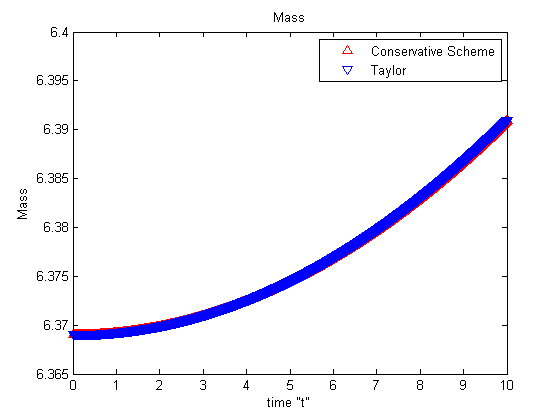
\includegraphics[width=\linewidth]{figures/Mass_bt3_c045_h005.png}
	\end{minipage}	
	\begin{minipage}[b]{0.49\linewidth}
		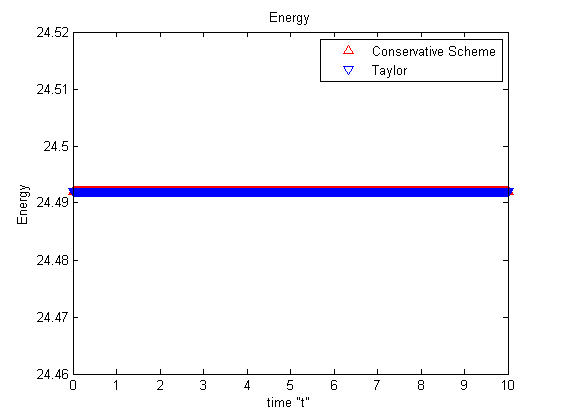
\includegraphics[width=\linewidth]{figures/Energy_bt3_c045_h005.png}
		
	\end{minipage}
\end{center}
The Mass (left) and Energy (right) of the solution for $\beta=3$, $c = 0.45$, $O(|h|^2 + \tau^2)$ and $T = 10$.

\begin{center}\vspace{0.4cm}
	\begin{minipage}[b]{0.49\linewidth}
		 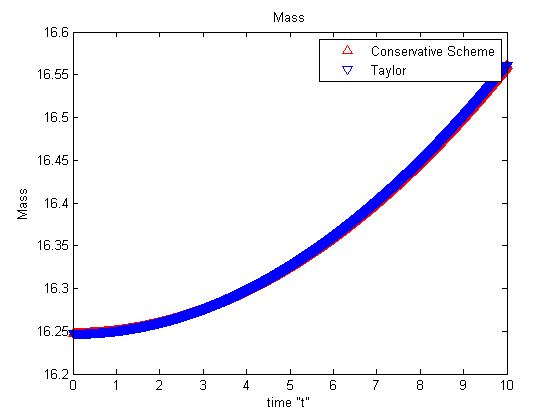
\includegraphics[width=\linewidth]{figures/Mass_bt1_c090_h010.png}
	\end{minipage}	
	\begin{minipage}[b]{0.49\linewidth}
		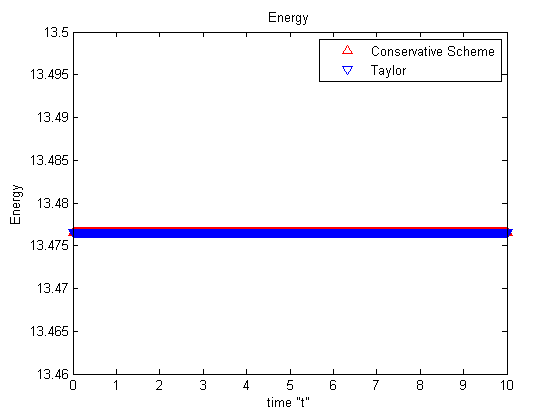
\includegraphics[width=\linewidth]{figures/Energy_bt1_c090_h010.png}
		
	\end{minipage}

\end{center}
The Mass (left) and Energy (right) of the solution for $\beta=1$, $c = 0.9$, $O(|h|^2 + \tau^2)$ and $T = 10$.

When comparing the Taylor and Conservative solutions one could see that they exhibit very near results. The convergence rates for the second order approximations are the same up to the first digit after the decimal point (see Table \ref{tableA} and Table \ref{tableC}). The same holds true for the energy convergence of both methods (see Tables \rf{table:B} and  \rf{tableD}) except for the case of $\beta = 1$ and $L_2$ norm but still the difference is less than $0.13$. Also the discrete integral vectors for both solution methods are the same as shown in Table \rf{tableE}. Table \rf{tableF} is a direct comparison in $L_2$ and Infinity norms between Taylor and Energy Saving methods. The results are very good as the obtained differences are very small compared to the solution maximum.

%E
\begin{table}[ht]
\centering
\small
		\begin{tabular}{||c|l|l|l|l||}
			\hline
			\hline
      \multirow{2  }{*}{FDS}        & \multirow{2  }{*}{$h$, $\tau$}  &   $uT_i - uE_i$  in $L_2$     &  $uT_i - uE_i$ in $L_\infty$ & \multirow{2  }{*}{$max|uE_i|$} \\
	                                        &                                                     &      difference                     &           difference                  &                                                       \\
   			\hline 
					\hline 
  $\beta=3$                   &0.2, 0.001         &  1.749e-05      &  1.965e-05  & 1.315448     \\
   c=0.45                        &0.1, 0.0005        &  8.109e-06       & 8.274e-06 &  1.862688     \\
     $O(h^2 + \tau^ 2)$ &0.05, 0.00025     & 2.460e-06         &2.502e-06  &   2.013184   \\
			\hline 
			\hline 
       $\beta=1$          &0.4, 0.002        & 0.009981     & 0.004560 & 0.656747   \\
                  c=0.9      &0.2, 0.001        & 0.005047      & 0.002373  & 0.673901   \\
  $O(h^2+ \tau^2)$ &0.1, 0.0005         & 0.002521      &0.001117 & 0.672231   \\
			\hline
	   \hline
			\hline 
		\end{tabular}
		\caption{Difference between obtained solutions with Energy Saving $uE$ and Taylor $uT$ methods using zero boundary condition and approximation errors $O(h^{2} + \tau^2 )$. Differences are measured in $L_2$ and $L_\infty$ norms.}
\label{tableF}
\end{table}

Notice that the final time $T=10$  is the same for all tables.

\begin{acknowledgments}
The work of the second author has been partially supported by
the Bulgarian Science Fund under grant K$\Pi$-06-H22/2.
\end{acknowledgments}

%\nocite{*}
%\bibliography{aipsamp}% Produces the bibliography via BibTeX.

\begin{thebibliography}{99} \normalsize

\bibitem{ref1} C.I. Christov, An energy-consistent dispersive shallow-water model,  {\it Wave Motion}, \textbf{34} (2001), 161-174.

\bibitem{ref4} I. Christov, C.I. Christov, Physical dynamics of quasi-particles in nonlinear wave equations,
{\it Physics Letters A}, \textbf{372}, Issue 4 (2008),  841-848.

\bibitem{ref5} J.K. Perring, T.H.R. Skyrme, A model unified field equation, {\it Nuclear Physics},  \textbf{31} (1962), 550-555.

\bibitem{ref13}   M. Christou, C.I. Christov,
Galerkin spectral method for the 2D solitary waves of Boussinesq paradigm equation,
In: {\it Applications of Mathematics in Technical and Natural Sciences, Sozopol (Bulgaria)},
\emph{AIP Conference Proceedings}, \textbf{1186}, Issue 1 (2009), 217-225.

\bibitem{ref14}  M. Christou, C.I. Christov,
Fourier Galerkin method for 2D solitons of Boussinesq equation,
{\it Mathematics and Computers in Simulation} \textbf{74} (2007), 82-92.

\bibitem{ref15} C.I. Christov, J. Choudhury, Perturbation solution for the 2D Boussinesq equation, {\it Mech. Res. Commun.}, \textbf{38} (2011), 274-281.

\bibitem{ref16}  K. Angelow, N. Kolkovksa, Numercal Study of Traveling Wave Solutions to 2D Boussinesq Equation, {\it Serdica J. Computing}, \textbf{13} (2019), 1-16.

\bibitem{ref20} Ch. Christov, D. Vasileva, N. Kolkovska, Numerical Realization of Unsteady Solutions for the 2D Boussinesq Paradigm Equation
{\it ???},
\emph{???}, \textbf{??} (2010), 395.

\bibitem{ref21} Chertok, Christov, Kurganov, Central-Upwind Schemes for the Boussinesq Paradigm Equations,
{\it ???},
\emph{???}, \textbf{??} (2010), 395.

\bibitem{ref22} K. Angelow, N. Kolkovska, A Multicomponent Alternating Direction Method for Numerical Solving of Boussinesq Paradigm Equation,
{\it ???},
\emph{???}, \textbf{??} (2010), 395.

\bibitem{ref23} M. Dimova, D. Vasileva, N. Kolkovska, Comparison of Two Numerical Approaches to Boussinesq Paradigm Equation,
{\it ???},
\emph{???}, \textbf{??} (2010), 395.

\bibitem{ref25} N. Kolkovska, Two families of finite difference schemes for multidimensional Boussinesq paradigm equation, In:
{\it Applications of Mathematics in Technical and Natural Sciences,  Sozopol (Bulgaria)},
\emph{AIP Conference Proceedings}, \textbf{1301} (2010), 395.

\bibitem{forn}
B.~Fornberg, Generation of Finite Difference Formulas on Arbitrarily Spaced Grids, 
Math. Comput., 51(1988),  699 -- 706.

%
\end{thebibliography}
\end{document}
%
% ****** End of file aipsamp.tex ******